\documentclass{article}

\textwidth=6.5in
\textheight=8.5in
\voffset=-54pt
\oddsidemargin=0in
\evensidemargin=0in
\setlength{\parskip}{8pt}
\setlength{\parindent}{0pt}

\usepackage[normalem]{ulem}

\usepackage{amsmath, amssymb}
\usepackage{ifthen}

\usepackage[inline]{enumitem}
\setlist{topsep=0pt, parsep=8pt}

\usepackage{xcolor}\convertcolorsUfalse
\usepackage[pdftex]{graphicx}

% change hyperref options
\PassOptionsToPackage{hyphens}{url}
\usepackage[bookmarks,colorlinks,linkcolor=black,citecolor=blue,pdfstartview=FitH,urlcolor=blue]{hyperref}
\hypersetup{pdfpagemode=UseNone}


\usepackage{graphicx}
\usepackage{multicol}
\usepackage{framed}
\usepackage{array}
\usepackage{diffcoeff}
\usepackage{icomma}

\usepackage{marginnote}
\usepackage[colorinlistoftodos]{todonotes}
\renewcommand{\marginpar}{\marginnote}

\usepackage{soul}

\usepackage{pgfplots}
\pgfplotsset{compat=1.18}  
\pgfplotscreateplotcyclelist{mycolor}{%
  black, blue, red, green!70!black,magenta,
  purple, cyan, orange
\pgfplotsset{
  cycle list name=mycolor,
  axis lines=middle,
  every axis plot/.style={no marks, thick},
  every axis/.style={
    enlarge x limits=false,
    enlarge y limits=auto,
    xlabel style={at={(current axis.right of origin)},anchor=west},
    ylabel style={at={(current axis.above origin)},anchor=south},
    % extra x and y ticks for asymptotes
    extra x tick style={grid=major, grid style={dashed,black}},
    extra y tick style={grid=major, grid style={dashed,black}},
    /pgf/number format/1000 sep={},
  },
  tick label style = {font=\footnotesize, fill=white, inner sep=0pt},
  xticklabel shift=1pt,    
  scaled ticks=false,
  scaled y ticks=false,
  unbounded coords=jump,
  samples=101,
  minor tick length=0,
  scatter/classes={
    open={mark=*,draw=black,fill=white, mark size=2, thin},
    closed={mark=*,draw=black,fill=black, mark size=2, thin}
  },
  compat=1.18
}


\usepackage{tikz}
\usetikzlibrary{
  % enables the snake paths
  decorations.pathmorphing,%
  % enables bigger arrows
  decorations.markings,%
  decorations.pathreplacing,%
  decorations.text,%
  calc,%
  patterns,%
  shapes.geometric,%
  arrows,
  decorations.shapes,
  positioning,
  plotmarks,
}
\tikzset{>=latex} % sets default arrow type in tikz
\tikzset{font=\small}

\interfootnotelinepenalty=10000
\renewcommand{\thefootnote}{(\arabic{footnote})}

\usepackage{multirow, bigdelim}

% change to \usepackage[sols]{handout} to see solutions
\usepackage[sols]{handout}
\renewcommand{\workshopnote}{CA Notes.}    

\newcommand\iscurrentenumi[1]{%
  \ifthenelse{\equal{#1}{\theenumi}}{}{#1}}
\setenumerate[1]{ref=\#\arabic*}
\setenumerate[2]{ref=\protect\iscurrentenumi{\theenumi}(\alph*)}
\newcommand\enumiiprefix[2]{%
  \ifthenelse{{\equal{#1}{\theenumi}}\AND{\equal{#2}{(\alph{enumii})}}}{}{}%
  \ifthenelse{{\equal{#1}{\theenumi}}\AND{\NOT{\equal{#2}{(\alph{enumii})}}}}{#2}{}%
  \ifthenelse{\equal{#1}{\theenumi}}{}{#1#2}%
}
\setenumerate[3]{ref=\protect\enumiiprefix{\theenumi}{(\alph{enumii})}\roman*}

\makeatletter

% underline links               
\let\@href=\href
\renewcommand{\href}[2]{\@href{#1}{\ul{#2}}}

\newcommand\iscurrentenumi[1]{%
  \ifthenelse{\equal{#1}{\theenumi}}{}{#1}}
\setenumerate[1]{ref=\#\arabic*}
\setenumerate[2]{ref=\protect\iscurrentenumi{\theenumi}(\alph*)}
\newcommand\enumiiprefix[2]{%
  \ifthenelse{{\equal{#1}{\theenumi}}\AND{\equal{#2}{(\alph{enumii})}}}{}{}%
  \ifthenelse{{\equal{#1}{\theenumi}}\AND{\NOT{\equal{#2}{(\alph{enumii})}}}}{#2}{}%
  \ifthenelse{\equal{#1}{\theenumi}}{}{#1#2}%
}
\setenumerate[3]{ref=\protect\enumiiprefix{\theenumi}{(\alph{enumii})}\roman*}

\definecolor{ideacolor}{rgb}{0.7,0,0}
\newcommand{\ideas}[1]{\color{ideacolor} #1 \color{black}}
\newcommand{\ideacolor}{maroon}

\newcommand{\outside}[1]{
    \fcolorbox{red}{white}{#1}
}

\newcommand{\inside}[1]{
    \fcolorbox{blue}{white}{#1}
}

\newlength{\tipmargin}
\makeatletter


\renewenvironment{framed}{
  \setlength{\tipmargin}{\textwidth-\linewidth}
  \advance\@totalleftmargin-\tipmargin
  \def\FrameCommand{\hspace{\tipmargin}\fbox}%
  \advance\linewidth\tipmargin
  \MakeFramed {\advance\hsize-\width \FrameRestore}%
}
{\endMakeFramed}

\makeatother

\newlength{\highlightwidth}
\newcommand{\highlight}[1]{\setlength{\highlightwidth}{\linewidth}%
  \addtolength{\highlightwidth}{-55pt}%
  \hspace{24pt}\begin{minipage}[t]{\highlightwidth} \setlength{\parskip}{8pt} #1 \end{minipage}\hspace{24pt}}

\definecolor{purple}{rgb}{0.5,0,1.0}

\newcommand\calculator{
  
\begin{tikzpicture}[x=0.15ex, y=0.15ex, baseline=1.5pt]
    \begin{scope}[thick]
      \draw (0, 0) -- (10, 0) -- (10, 14) -- (0, 14) -- cycle;
      \foreach \x in {10/3, 20/3}
      {
        \draw (\x, 0) -- (\x, 10);
      }
      \foreach \y in {10/3, 20/3, 10}
      {
        \draw (0, \y) -- (10, \y);
      }
    \end{scope}
  \end{tikzpicture}
}
\newcommand{\calcitem}{\refstepcounter{enum\romannumeral\@enumdepth}%
\item[\calculator \csname labelenum\romannumeral\@enumdepth\endcsname]}

\makeatother

\definecolor{purple}{rgb}{0.5,0,1.0}

\newcommand{\doedfinity}[2][\newpage]{
  \begin{problem}[#1]
    Do the Edfinity assignment ``Problem Set #2''.

    We encourage you to write down any scratch work here, as well as
    things you want your future self to remember. Nothing you write
    here will be graded; it's just for you!
  \end{problem}
}

\newcommand{\psrnewpage}{\newpage}
\newcommand{\psreflection}[2][]{

  \ifthenelse{\not\equal{#1}{nocite}}{
    \begin{enumerate}[resume]
    \item
      \begin{problem}[1in]
        Please cite any help you got on this problem set:
        \begin{itemize}[nosep]
        \item If you worked with other students, please list their names here.
        \item If you used resources other than those on our Canvas site, please list them here.
        \end{itemize}
      \end{problem}

    \end{enumerate}
  }

  \probonly{%
    #2

    \psrnewpage

    \emph{Reflection space.} It's a good habit to take a few minutes at the end of each pset to reflect on what you learned and jot down notes to your future self. Here are a few reflection questions to get you started. Nothing you write here will be graded; it's just for you!
    \begin{itemize}
    \item Take a few minutes to look back at the problems. How could you explain to someone else how to do each problem? What was your strategy, and how did you know to use that strategy? If there are problems where you don't feel able to answer this, write down which ones they are. Come back to them in a few days when we post the homework solutions!

      \vspace{1.5in}

    \item Take a look back at the learning objectives on today's worksheet; how are you feeling about each one? If there are ones you know you need more practice with, write those down here.

      \vspace{1.5in}

    \item What did you find most challenging about this material? Do you have any lingering questions about it? If so, write them down here so you don't forget them. At some point, stop by office hours or MQC to ask!

      \vfill
    \end{itemize}      
  }
}

\usepackage{fancyhdr}
\lhead{\textcolor{white}{This content is protected and may not be shared, uploaded, or distributed.}}
\rhead{}
\rfoot{\vspace*{\fill}\footnotesize\textcopyright{} \emph{Harvard Math Ma}}
\renewcommand{\headrulewidth}{0pt}
\pagestyle{fancy}

\begin{document}

\begin{center}
  \large\textsc{Problem Set 33 - Derivative Review (Chain Rule, Day 2)}
\end{center}

\solonly{
  \begin{framed}
    \emph{Note:} The solutions are color-coded according to the rule being
    used.  Two boxes in green indicate a product of two terms, which
    requires the Product Rule.  A blue box inside a red box means the
    Chain Rule is about to be used, with the blue box giving the inside
    function.  A purple box shows a constant multiple.  An orange box
    shows an expression that can be simplified using log or exponent
    rules.
  \end{framed}
}

\textit{For a reference on the Chain Rule, read the examples on pages 518 - 519 in the \href{https://canvas.harvard.edu/courses/138327/files/20608911?wrap=1}{Gottlieb textbook}. (This is the
  start of \S 16.1).  In particular, be sure that you understand examples 16.4 and 16.5 before attempting the problems below. As always, you must show your work or explain your reasoning for full credit!}

\begin{enumerate}
\item
\begin{grading}
    16 points. 2 points each for parts (a)i-iv, and 3 points each for parts (a)v. and (a)vi. 2 points for part (b). As usual, if students only write a final answer without any work or ideas shown, they should not receive any credit.
\end{grading}


  \begin{enumerate}
  \item
Differentiate each of the following functions with respect to $x$. It may be useful to
    first simplify or rewrite the given function.  (Not all of them require the Chain Rule!)

      \begin{enumerate}
      \item
        \begin{problem}[\vfill]
          $e^{x^2}$
        \end{problem}

      \begin{solution}
        $\displaystyle \frac{d}{dx}
        \left(\fcolorbox{red}{white}{$\displaystyle e^ {
              \fcolorbox{blue}{white}{$\displaystyle x^ { 2} $}} $}\right)
        = {} e^ { x^ { 2} } \cdot 2 x$.
      \end{solution}

    \item
      \begin{problem}[\vfill]
        $(e^x)^2$
      \end{problem}

      \begin{solution}
        $(e^x)^2 = e^{2x}$, so the derivative of this is $2 e^ { 2 x}$.
      \end{solution}

    \item
      \begin{problem}[\vfill]
        $\sqrt{\ln x + 1}$
      \end{problem}

      \begin{solution}
        \begin{align*}
          \frac{d}{dx} \left(\fcolorbox{red}{white}{$\displaystyle \fcolorbox{blue}{white}{$\displaystyle \left(\ln x+ 1\right)$}^ { \frac{1}{2}} $}\right) = {} & \frac{1}{2} \left(\ln x+ 1\right)^ { -\frac{1}{2}} \cdot \frac{d}{dx}\left(\ln x+ 1\right) \\
          = {} & \frac{1}{2} \left(\ln x+ 1\right)^ { -\frac{1}{2}} \cdot
          \frac{1}{x}
        \end{align*}
      \end{solution}

    \item
      \begin{problem}[\vfill\newpage]
        $\ln \sqrt{x + 1}$
      \end{problem}

      \begin{solution}
        \begin{align*}
          \frac{d}{dx} \left(\fcolorbox{orange}{white}{$\displaystyle \ln\left(\sqrt{x+ 1}\right)$}\right) = {} & \frac{d}{dx} \left(\fcolorbox{purple}{white}{$\displaystyle \frac{1}{2}$} \ln\left(x+ 1\right)\right) \\
          = {} & \frac{1}{2}\cdot \frac{d}{dx} \left(\fcolorbox{red}{white}{$\displaystyle \ln\left(\fcolorbox{blue}{white}{$\displaystyle x+ 1$}\right)$}\right) \\
          = {} & \frac{1}{2}\cdot \left(\frac{1}{x+ 1}\cdot 1\right)
        \end{align*}
      \end{solution}

    \item % 16.1.6

    \begin{problem}[\vfill]
     $  e^{5x}(1+2x)^6$  

      \emph{Hint:} The Chain Rule is not the first rule you need.  What
      is?
    \end{problem}

    \begin{solution}
      \begin{align*}
        \frac{d}{dx} \left(\fcolorbox{green}{white}{$\displaystyle  e^ { 5 x} $}\cdot \fcolorbox{green}{white}{$\displaystyle  \left(1+ 2 x\right)^ { 6} $}\right) = {} & e^ { 5 x} \cdot \frac{d}{dx} \left(\fcolorbox{red}{white}{$\displaystyle \fcolorbox{blue}{white}{$\displaystyle  \left(1+ 2 x\right)$}^ { 6 } $}\right)+ 5 e^ { 5 x} \left(1+ 2 x\right)^ { 6}  \\
        = {} & e^ { 5 x} \left(6 \left(1+ 2 x\right)^ { 5} \cdot 2\right)+ 5 e^ { 5 x} \left(1+ 2 x\right)^ { 6} 
      \end{align*}
    \end{solution}

      \item
    \begin{problem}[\vfill]
      If $\displaystyle f(x) = \ln\left(\frac{\left(2 x+
            3\right)^2}{\left(5 x+ 2\right)^4 \left(x^2+
            1\right)}\right)$, find $f'(x)$.

      \emph{Hint:} This will be easier if you simplify $f(x)$
      using log rules before differentiating. 
    \end{problem}

    \begin{solution}
      \begin{align*}
        & \frac{d}{dx} \left(\fcolorbox{orange}{white}{$\displaystyle \ln\left(\frac{\left(2 x+ 3\right)^2}{\left(5 x+ 2\right)^4 \left(x^2+ 1\right)}\right)$}\right) \\
        = {} & \frac{d}{dx} \left(\fcolorbox{purple}{white}{$\displaystyle 2$}\cdot \ln\left(2 x+ 3\right)\right)- \frac{d}{dx} \left(\fcolorbox{purple}{white}{$\displaystyle 4$}\cdot \ln\left(5 x+ 2\right)\right)-\frac{d}{dx} \left(\fcolorbox{red}{white}{$\displaystyle \ln\left(\fcolorbox{blue}{white}{$\displaystyle x^ { 2} + 1$}\right)$}\right) \\
        = {} & 2\cdot \frac{d}{dx} \left(\fcolorbox{red}{white}{$\displaystyle \ln\left(\fcolorbox{blue}{white}{$\displaystyle 2 x+ 3$}\right)$}\right)-4\cdot \frac{d}{dx} \left(\fcolorbox{red}{white}{$\displaystyle \ln\left(\fcolorbox{blue}{white}{$\displaystyle 5 x+ 2$}\right)$}\right)-\left(\frac{1}{x^ { 2} + 1}\cdot \left(2 x\right)\right) \\
        = {} & 2 \cdot \frac{1}{2 x+ 3}\cdot 2-4 \cdot \frac{1}{5 x+ 2}\cdot 5-\frac{1}{x^ { 2} + 1}\cdot 2 x
      \end{align*}
    \end{solution}

    \end{enumerate}
    \probonly{}

  \item
    \begin{problem}[1in]
      \textbf{Reflect Back.}  For two of the functions in
      {{{{\#1}}(a)}}, you can simplify the function before
      differentiating; which two?
    \end{problem}

\end{enumerate}
    \item

\begin{grading}
20 points. 4 points for each part. 
\end{grading}

 % 16.2.5

  Find $y'$, simplifying the expressions first where useful. You need not simplify your final
  answers.

  \emph{General advice: Before you start differentiating, take a moment to
    see if you can rewrite the function in a way that makes the
    differentiation easier.  (Example 16.8 on page 525 in the \href{https://canvas.harvard.edu/courses/138327/files/20608911?wrap=1}{textbook} is a good example
    of this.)  Being flexible in your problem-solving tactics can save you
    a lot of time in problems like this (and is also a skill that will
    serve you well in any endeavor).}

  \begin{enumerate}[topsep=0pt]
  \item
    \begin{problem}[\vfill\newpage]
      $y = \displaystyle \frac{e^{1/x}}{x^2}$
    \end{problem}

    \begin{solution}
      \begin{align*}
        \frac{d}{dx} \left(\fcolorbox{green}{white}{$\displaystyle  e^ { x^ { -1} } $}\cdot \fcolorbox{green}{white}{$\displaystyle  x^ { -2} $}\right) = {} & e^ { x^ { -1} } \cdot \left(-2\cdot x^ { -3} \right)+ \frac{d}{dx} \left(\fcolorbox{red}{white}{$\displaystyle e^ { \fcolorbox{blue}{white}{$\displaystyle x^ { -1} $}} $}\right)\cdot x^ { -2}  \\
        = {} & e^ { x^ { -1} } \cdot \left(-2\cdot x^ { -3} \right)+ \left(e^ { x^ { -1} } \cdot -x^ { -2} \right)\cdot x^ { -2} 
      \end{align*}
    \end{solution}
    
  \item % 16.1.20
    \begin{problem}[\vfill]
     $\displaystyle y = x\ln \left(\frac{x}{x^2+1}\right)$ Hint: Simplify this expression using log rules before you differentiate.
    \end{problem}

    \begin{solution}
      This is easiest if we first use log rules to rewrite $y$ as $y = x
      \left[ \ln x - \ln (x^2 + 1) \right]$.  Then,
      \begin{align*}
        \frac{dy}{dx} &= \frac{d}{dx}
        \left(\fcolorbox{green}{white}{$\displaystyle x$}\cdot
          \fcolorbox{green}{white}{$\displaystyle \left[\ln x-\ln\left(x^2
                + 1\right)\right]$}\right) \\
        &= x \left(\frac{1}{x}-\frac{d}{dx}
          \left(\fcolorbox{red}{white}{$\displaystyle
              \ln\left(\fcolorbox{blue}{white}{$\displaystyle x^ { 2} +
                  1$}\right)$}\right)\right)+ 1 \left[\ln x-\ln\left(x^ {
              2} + 1\right)\right] \\
        &= x \left(\frac{1}{x}-\frac{1}{x^ { 2} + 1}\cdot 2 x\right)+ \ln
        x-\ln\left(x^ { 2} + 1\right)
      \end{align*}
    \end{solution}

  \item 
    \begin{problem}[\vfill\newpage]
      $y = (1 - \ln x)^{5/4}$
    \end{problem}

    \begin{solution}
      \begin{align*}
        \frac{d}{dx} \fcolorbox{red}{white}{$\left(
            \fcolorbox{blue}{white}{$1-\ln x$} \right)^{5/4}$} =
        \frac{5}{4}\left(1-\ln x\right)^{1/4} \cdot \left( -\frac{1}{x}
        \right)
      \end{align*}
    \end{solution}

  \item
    \begin{problem}[\vfill]
     $\displaystyle y = \frac{6 x^2}{\ln 3} +
        \frac{1}{\sqrt{x+ \ln x}}$ 
    \end{problem}

    \begin{solution}
      \begin{align*}
        \frac{d}{dx}\left( \frac{6 x^2}{\ln 3} +
        \frac{1}{\sqrt{x+ \ln x}} \right) = {} & \frac{d}{dx}
        \left(\fcolorbox{purple}{white}{$\displaystyle \frac{6}{\ln
              3}$}\cdot x^ { 2} \right)+ \frac{d}{dx}
        \left(\fcolorbox{red}{white}{$\displaystyle
            \fcolorbox{blue}{white}{$\displaystyle (x+ \ln x)$}^ {
              -\frac{1}{2}} $}\right) \\ 
        = {} & \frac{6}{\ln 3} \left(2x
        \right)-\frac{1}{2} \left(x+ \ln x\right)^ { -\frac{3}{2}}
        \cdot \frac{d}{dx}\left(x+ \ln x\right) \\ 
        = {} & \frac{6}{\ln 3} \left(2x
        \right)-\frac{1}{2} \left(x+ \ln x\right)^ { -\frac{3}{2}}
        \cdot \left(1+ \frac{1}{x}\right) 
      \end{align*}
    \end{solution}

  \item
    \begin{problem}[\vfill\newpage]
      $y = \left[ \ln \sqrt{1 - x} \right]^{-3.5}$ Hint: There is one simplification that you can do and several tempting maneuvers that you can't do!
    \end{problem}

    \begin{solution}
      This is easiest if we first use log rules to simplify $y$ a bit:
      $\ln \sqrt{1 - x} = \ln \left[ (1 - x)^{1/2} \right] = \frac{1}{2}
      \ln (1 - x)$, so we can rewrite
      \[ y = \left( \frac{1}{2} \ln (1 - x) \right)^{-3.5} = \left(
        \frac{1}{2} \right)^{-3.5} \left[ \ln (1 - x) \right]^{-3.5}.\]
      Since $\left(
        \frac{1}{2} \right)^{-3.5}$ is a constant,
      \begin{align*}
        y' &= \left( \frac{1}{2} \right)^{-3.5} \frac{d}{dx}
        \left(\fcolorbox{red}{white}{$\displaystyle
            \fcolorbox{blue}{white}{$\displaystyle
              \left[\ln\left(1-x\right)\right]$}^{-3.5} $}\right) \\
        &= \left( \frac{1}{2} \right)^{-3.5} (-3.5) \left[\ln(1-x)\right]^
        { -4.5} \cdot \frac{d}{dx} 
        \left(\fcolorbox{red}{white}{$\displaystyle
            \ln\left(\fcolorbox{blue}{white}{$\displaystyle
                1-x$}\right)$}\right) \\ 
        &= \left( \frac{1}{2} \right)^{-3.5} (-3.5) \left[\ln(1-x)\right]^
        { -4.5} \cdot 
        \left(\frac{1}{1-x}\cdot -1\right) \\
        &= \left( \frac{1}{2} \right)^{-3.5} \frac{3.5}{1 - x}
        \left[\ln(1-x)\right]^ { -4.5} 
      \end{align*}
    \end{solution}
  \end{enumerate}  
    \pspace{\newpage}

    \begin{solution}
      The functions in {\enumiiprefix {{{\#1}}}{(a)}ii} and
      {\enumiiprefix {{{\#1}}}{(a)}iv}.
    \end{solution}

 

%%%%%%
\item 

% 16.1.27, 16.1.28 mashed together
\begin{grading}
    24 points. Points for parts (a)-(i) should be distributed as follows:\\
    3/2/2/2/2/4/2/5/2. For part (c), they need to show that $f(-x)=f(x)$.
\end{grading}

    Let $f(x) = e^{-x^2}$.
    This is an important function to become familiar with as it comes up
    frequently in both probability and statistics \footnote{The function $e^{-x^2}$ is used frequently in both probability
    and statistics because, with some minor adjustments, it gives us a
    normal distribution curve (i.e., a bell curve).}. We explore it below.
    
  \begin{enumerate}

  \item Which of the following are equal to $e^{-x^2}$?  Identify
    \emph{all} correct answers.  
      \begin{enumerate}[label=\protect\maybecircle{\roman*.}]
      \begin{multicols}{3}
      \circleitem $\frac{1}{e^{x^2}}$
      \plainitem $e^{-2x}$
      \circleitem $(e^{-x})^x$ 
      \circleitem $\left({\frac{1}{e^x}}\right)^x$
      \plainitem $\left(\frac{1}{e^x}\right)^2$
      \plainitem $(e^{-x})^2$
      \end{multicols}
      \end{enumerate}      
    (You should have found 3 correct choices.)

  \item
    \begin{problem}[\vfill]
      What is the domain of $f$?
    \end{problem}

    \begin{solution}
      All real numbers.  (No matter what $x$ is, $e^{-x^2}$ is defined.) 
    \end{solution}

  \item
    \begin{problem}[\vfill]
      Is $f$ an even function, an odd function, or neither?
    \end{problem}

    \begin{solution}
     To determine this, we want to see how $f(-x)$ relates to
        $f(x)$.  If $f(-x) = f(x)$, then $f$ is even; if $f(-x) = -f(x)$,
        then $f$ is odd; otherwise, $f$ is neither.

      Here, $f(-x) = e^{-(-x)^2} = e^{-x^2} = f(x)$, so $f$ is
      \fbox{even}.
    \end{solution}

  \item
    \begin{problem}[\stretch{2}]
      Find the derivative of $f(x) = e^{-x^2}$. 
    \end{problem}

    \begin{solution}
      $f'(x) = \displaystyle \frac{d}{dx}
      \left(\fcolorbox{red}{white}{$\displaystyle e^ {
            \fcolorbox{blue}{white}{$\displaystyle -x^ { 2} $}} $}\right)
      = {} e^ { -x^ { 2} } \cdot \left(-2 x\right)$.
    \end{solution}    

  \item
    \begin{problem}[\nstretch{2}]
      For what values of $x$ is $f$ increasing?
    \end{problem}

    \begin{solution}
      To answer this, let's make a sign chart for $f'$, since we
        know that the sign of $f'$ tells us whether $f$ is increasing or
        decreasing.

      First, we'll figure out where $f'(x)$ is 0.  That is, we want to
      solve $-2x e^{-x^2} = 0$.  If a product of terms is 0, at least one
      of the terms is 0, so either $x = 0$ or $e^{-x^2} = 0$; the latter
      is impossible, so the only critical point of $f$ is $x = 0$.
      Testing a value of $x$ greater than 0 and a value of $x < 0$ gives
      us the following sign chart:
      \begin{center}
        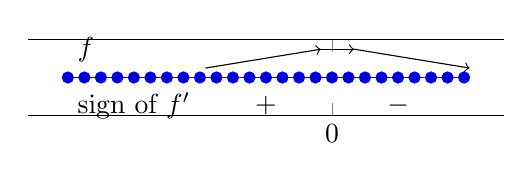
\begin{tikzpicture}
          \begin{axis}[axis y line=none, x axis line style={-}, xtick={0.}, xticklabels={$0$}, ymin=-2, ymax=2, height=1in, width=3in, clip=false]
            \addplot+[domain=-4:2]{0};
            \draw (axis cs: -4, 1.5) node[right] {$f$};
            \draw (axis cs: -4, -1.5) node[right] {sign of $f'$};
            \draw (axis cs: -1, -1.5) node{$+$};
            \draw (axis cs: 1, -1.5) node{$-$};
            \draw[->, xshift=2pt] (-2,0.5) -- (-0.25,1.5);
            \draw[->, xshift=2pt] (-0.25,1.5) -- (0.25,1.5);
            \draw[->, xshift=2pt] (0.25,1.5) -- (2,0.5);
          \end{axis}
        \end{tikzpicture}
      \end{center}
      
      (For example, $f'(-1) = 2 e^{-1} > 0$ and $f'(1) = -2 e^{-1} < 0$.)
      So, $f$ is increasing on $\boxed{(-\infty, 0)}$.
    \end{solution}

  \item
    \begin{problem}[\vfill]
      For what values of $x$ is $f$ concave up?
    \end{problem}

    \begin{solution}
      To answer this, let's make a sign chart for $f''$, since we
        know that the sign of $f''$ tells us whether $f$ is concave up or
        concave down.

      First, we'll compute $f''$:
      \begin{align*}
        f''(x) = {} & \frac{d}{dx}
        \left(\fcolorbox{purple}{white}{$\displaystyle -2$}\cdot x\cdot e^
          { -x^ { 2} } \right) \\
        = {} & -2\cdot \frac{d}{dx} \left(\fcolorbox{green}{white}{$\displaystyle x$}\cdot \fcolorbox{green}{white}{$\displaystyle e^ { -x^ { 2} } $}\right) \\
        = {} & -2 \left(x\cdot \frac{d}{dx} \left(\fcolorbox{red}{white}{$\displaystyle e^ { \fcolorbox{blue}{white}{$\displaystyle -x^ { 2} $}} $}\right)+ e^ { -x^ { 2} } \right) \\
        = {} & -2 \left(x\cdot \left(e^ { -x^ { 2} } \cdot \left(-2
              x\right)\right)+ e^ { -x^ { 2} } \right) \\
        = {} & -2 e^{-x^2} (-2x^2 + 1)
      \end{align*}
      This is equal to 0 when $-2x^2 + 1 = 0$, which happens when $x = \pm
      \dfrac{1}{\sqrt{2}}$.  We can determine where $f''$
      is positive and negative and add the information to
      our sign chart:

      \begin{center}
        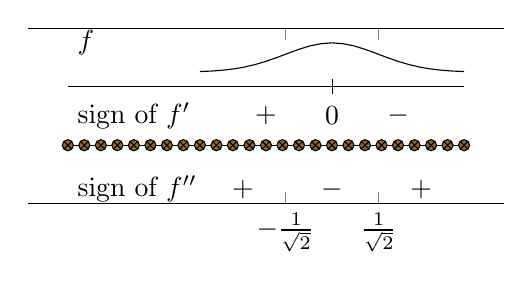
\begin{tikzpicture}
          \begin{axis}[axis y line=none, x axis line style={-}, xtick={-0.707107, 0.707107}, xticklabels={$-\frac{1}{\sqrt{2}}$, $\frac{1}{\sqrt{2}}$}, ymin=-2,
          ymax=4, height=1.5in, width=3in]
            \addplot[black, domain=-4:2]{2};
            \draw[black,line width=0.1pt] (0,1.75) -- (0,2.25); 
            \draw (0,1) node {$0$};
            \draw (axis cs: -4, 3.5) node[right] {$f$};
            \draw (axis cs: -4, 1) node[right]
            {sign of $f'$};
            \draw (axis cs: -1, 1) node{$+$};
            \draw (axis cs: 1, 1) node{$-$};

            \addplot[black,thin,domain=-2:2]{e^(-x^2)+2.5};
            
            \addplot+[black, domain=-4:2]{0};
            \draw (axis cs: -4, -1.5) node[right] {sign of $f''$};
            \draw (axis cs: -1.35, -1.5) node{$+$};
            \draw (axis cs: 0., -1.5) node{$-$};
            \draw (axis cs: 1.35, -1.5) node{$+$};
          \end{axis}
        \end{tikzpicture}
      \end{center}
      So, $f$ is concave up on \fbox{$\displaystyle \left(-\infty, -
          \frac{1}{\sqrt{2}} \right)$ and $\displaystyle \left(
          \frac{1}{\sqrt{2}}, \infty \right)$}.
    \end{solution}

  \item
    \begin{problem}[\vfill]
      What is $\displaystyle \lim_{x \to \infty} e^{-x^2}$?  What is
      $\displaystyle \lim_{x \to -\infty} e^{-x^2}$?
    \end{problem}

    \begin{solution}
      For $\displaystyle \lim_{x \to \infty} e^{-x^2}$, we think about
      what happens to $e^{-x^2}$ if we plug in a really huge number for
      $x$.  If $x$ is really huge, then the exponent $-x^2$ is a huge
      negative number, and $e$ raised to a huge negative number is close
      to 0.  So, $\displaystyle \lim_{x \to \infty} e^{-x^2} = 0$.

      Similarly, $\displaystyle \lim_{x \to -\infty} e^{-x^2} = 0$. 
    \end{solution}

  \item

    \begin{grading}
      If a student's graph is inconsistent with anything he/she has done
      in the previous parts, please point that out.  One thing we really
      want students to work on this semester is consistency within a
      problem. 
    \end{grading}

    \begin{problem}[\nstretch{2}]
      Use what you've done so far in this problem to sketch the graph of
      $f(x)$.  Label the coordinates of any local minima and local
      maxima.

      \probonly{\emph{Make sure your graph is consistent with everything
          that you've found in this problem.  Does it have the right
          symmetry?  Does it increase and decrease on the appropriate
          intervals?  Is it concave up and concave down on the appropriate
          intervals?  After you've checked by hand, you are also welcome
          to check your graph using a calculator or computer;
          \url{https://www.desmos.com/calculator} or \url{https://www.wolframalpha.com/} are good options.}}
    \end{problem}

    \begin{solution}
      Here is the graph; it has one local maximum, at $(0, 1)$, and no
      local minima.
      \begin{center}
        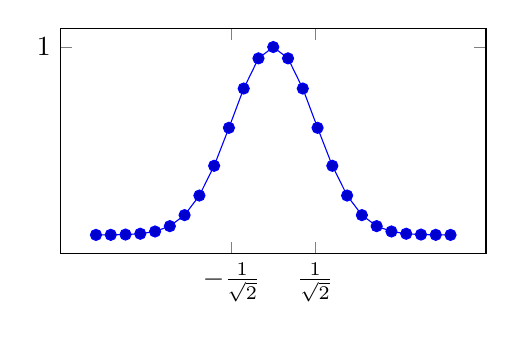
\begin{tikzpicture}
          \begin{axis}[xtick={-0.707, 0.707},
            xticklabels={$-\frac{1}{\sqrt{2}}$, $\frac{1}{\sqrt{2}}$},
            ytick=1, width=2.75in, height=1.75in]
            \addplot+[domain=-3:3] {e^(-x^2)};
          \end{axis}
        \end{tikzpicture}
      \end{center}
    \end{solution}

  \item
    \begin{problem}[\vfill]
      Does $f$ have an absolute maximum value?  If so, what?  Does
      $f$ have an absolute minimum value?  If so, what?
    \end{problem}

    \begin{solution}
      We can see from our graph that $f$ has an absolute maximum at $x =
      0$, and the absolute maximum value is 1.  $f$ does not have an
      absolute minimum value.
    \end{solution}

  \end{enumerate}

\item 
\begin{grading}
    4 points. 2 points for the correct choices, 2 points for the explanations.
\end{grading}
 \textbf{Reflect Back.}

  \begin{problem}[\vfill]
    Which two of the following functions would absolutely REQUIRE the Chain Rule to differentiate? Briefly explain why the other two functions do NOT require the Chain Rule.
      \begin{enumerate}[label=\protect\maybecircle{\Alph*.},topsep=0pt]
      \plainitem $\displaystyle f(x) =\frac{1}{ \ln(4x^9)}$
      \plainitem $f(x) = \ln [(2x)^8]$
      \circleitem $f(x) = [\ln(1+x)]^3$
      \circleitem $f(x) = \ln(x+x^2)$
      \end{enumerate}
    
  \end{problem}

  \begin{solution}
      C and D both require the Chain Rule.

  For C,
  \begin{align*}
      
  
    \diff*{\left(\outside{$\inside{$\ln(1+x)$}^3$}\right)}{x}
    &= 3\left[\ln(1+x)\right]^2 \cdot \dfrac{d}{dx}\left(\outside{$\ln\left(\inside{$1+x$}\right)$}\right) \\
    &= 3\left[\ln(1+x)\right]^2 \cdot \dfrac{1}{1+x} \cdot 1
  \end{align*}

  For D,
  \begin{align*}
    \diff*{\left(\outside{
    $\ln\left(\inside{$x+x^2$}\right)$}\right)}{x}
    &= \frac{1}{x+x^2}\cdot(1+2x)
  \end{align*}

  A can be done using the Quotient Rule and properties of
  logarithms. It will be easier if we first differentiate
  $\ln(4x^9)$.

  \[\diff*{\ln(4x^9)}{x}=\diff*{\ln(4)}{x} + \diff*{9\ln x}{x}
  = \frac{9}{x}\]

  Then we can use the Quotient Rule.
  
    \begin{align*}
    \diff*{\left(\frac{1}{\ln(4x^9)}\right)}{x}
    &= \frac{\diff*{1}{x} \cdot \ln(4x^9)- 1 \cdot 
    \diff*{\ln(4x^9)}{x}}{[\ln(4x^9)]^2} \\
    &= \frac{0 \cdot \ln(4x^9) - 1 \cdot \frac{9}{x}}
    {[\ln(4x^9)]^2} \\
    &= \frac{-9}{x[\ln(4x^9)]^2}
    \end{align*}

 B can be done using properties of logarithms.

 \begin{align*}
    \diff*{\ln[(2x)^8]}{x} &= \diff*{8\ln(2x)}{x} \\
    &= 8\left(\diff*{\ln 2}{x} + \diff*{\ln x}{x}\right) \\
    &= \dfrac{8}{x}
    \end{align*}
 
  \end{solution}



 \end{enumerate}
 


\psreflection{For next class, read \S 14.1 - 14.3.}
\end{document}
